\documentclass{psico-latex-essay}

\usepackage{graphicx}
\usepackage{amsmath}
\usepackage{natbib}
\usepackage{lipsum}

\bibliographystyle{plainnat}

\graphicspath{{images/}}

\author{Guilherme Dias}

\title{Psico \LaTeX\ Essay}

\begin{document}
\maketitle

\lipsum[1-1][1-5]

\section{Level 1 Heading}
\lipsum[1-1][1-5]

\subsection{Level 2 Heading}
\lipsum[1-1][1-5]

\subsubsection{Level 3 Heading}
\lipsum[1-1][1-5]
As we can see in the equation~\ref{eq:integral},

\begin{align}
  \int_{0}^{1} f(x) dx
  \label{eq:integral}
\end{align}

\paragraph{Level 4 Heading}
\lipsum[1-1][1-5]
As we can see in the figure~\ref{fg:graphic}.

\begin{figure}[ht]
  \centering
  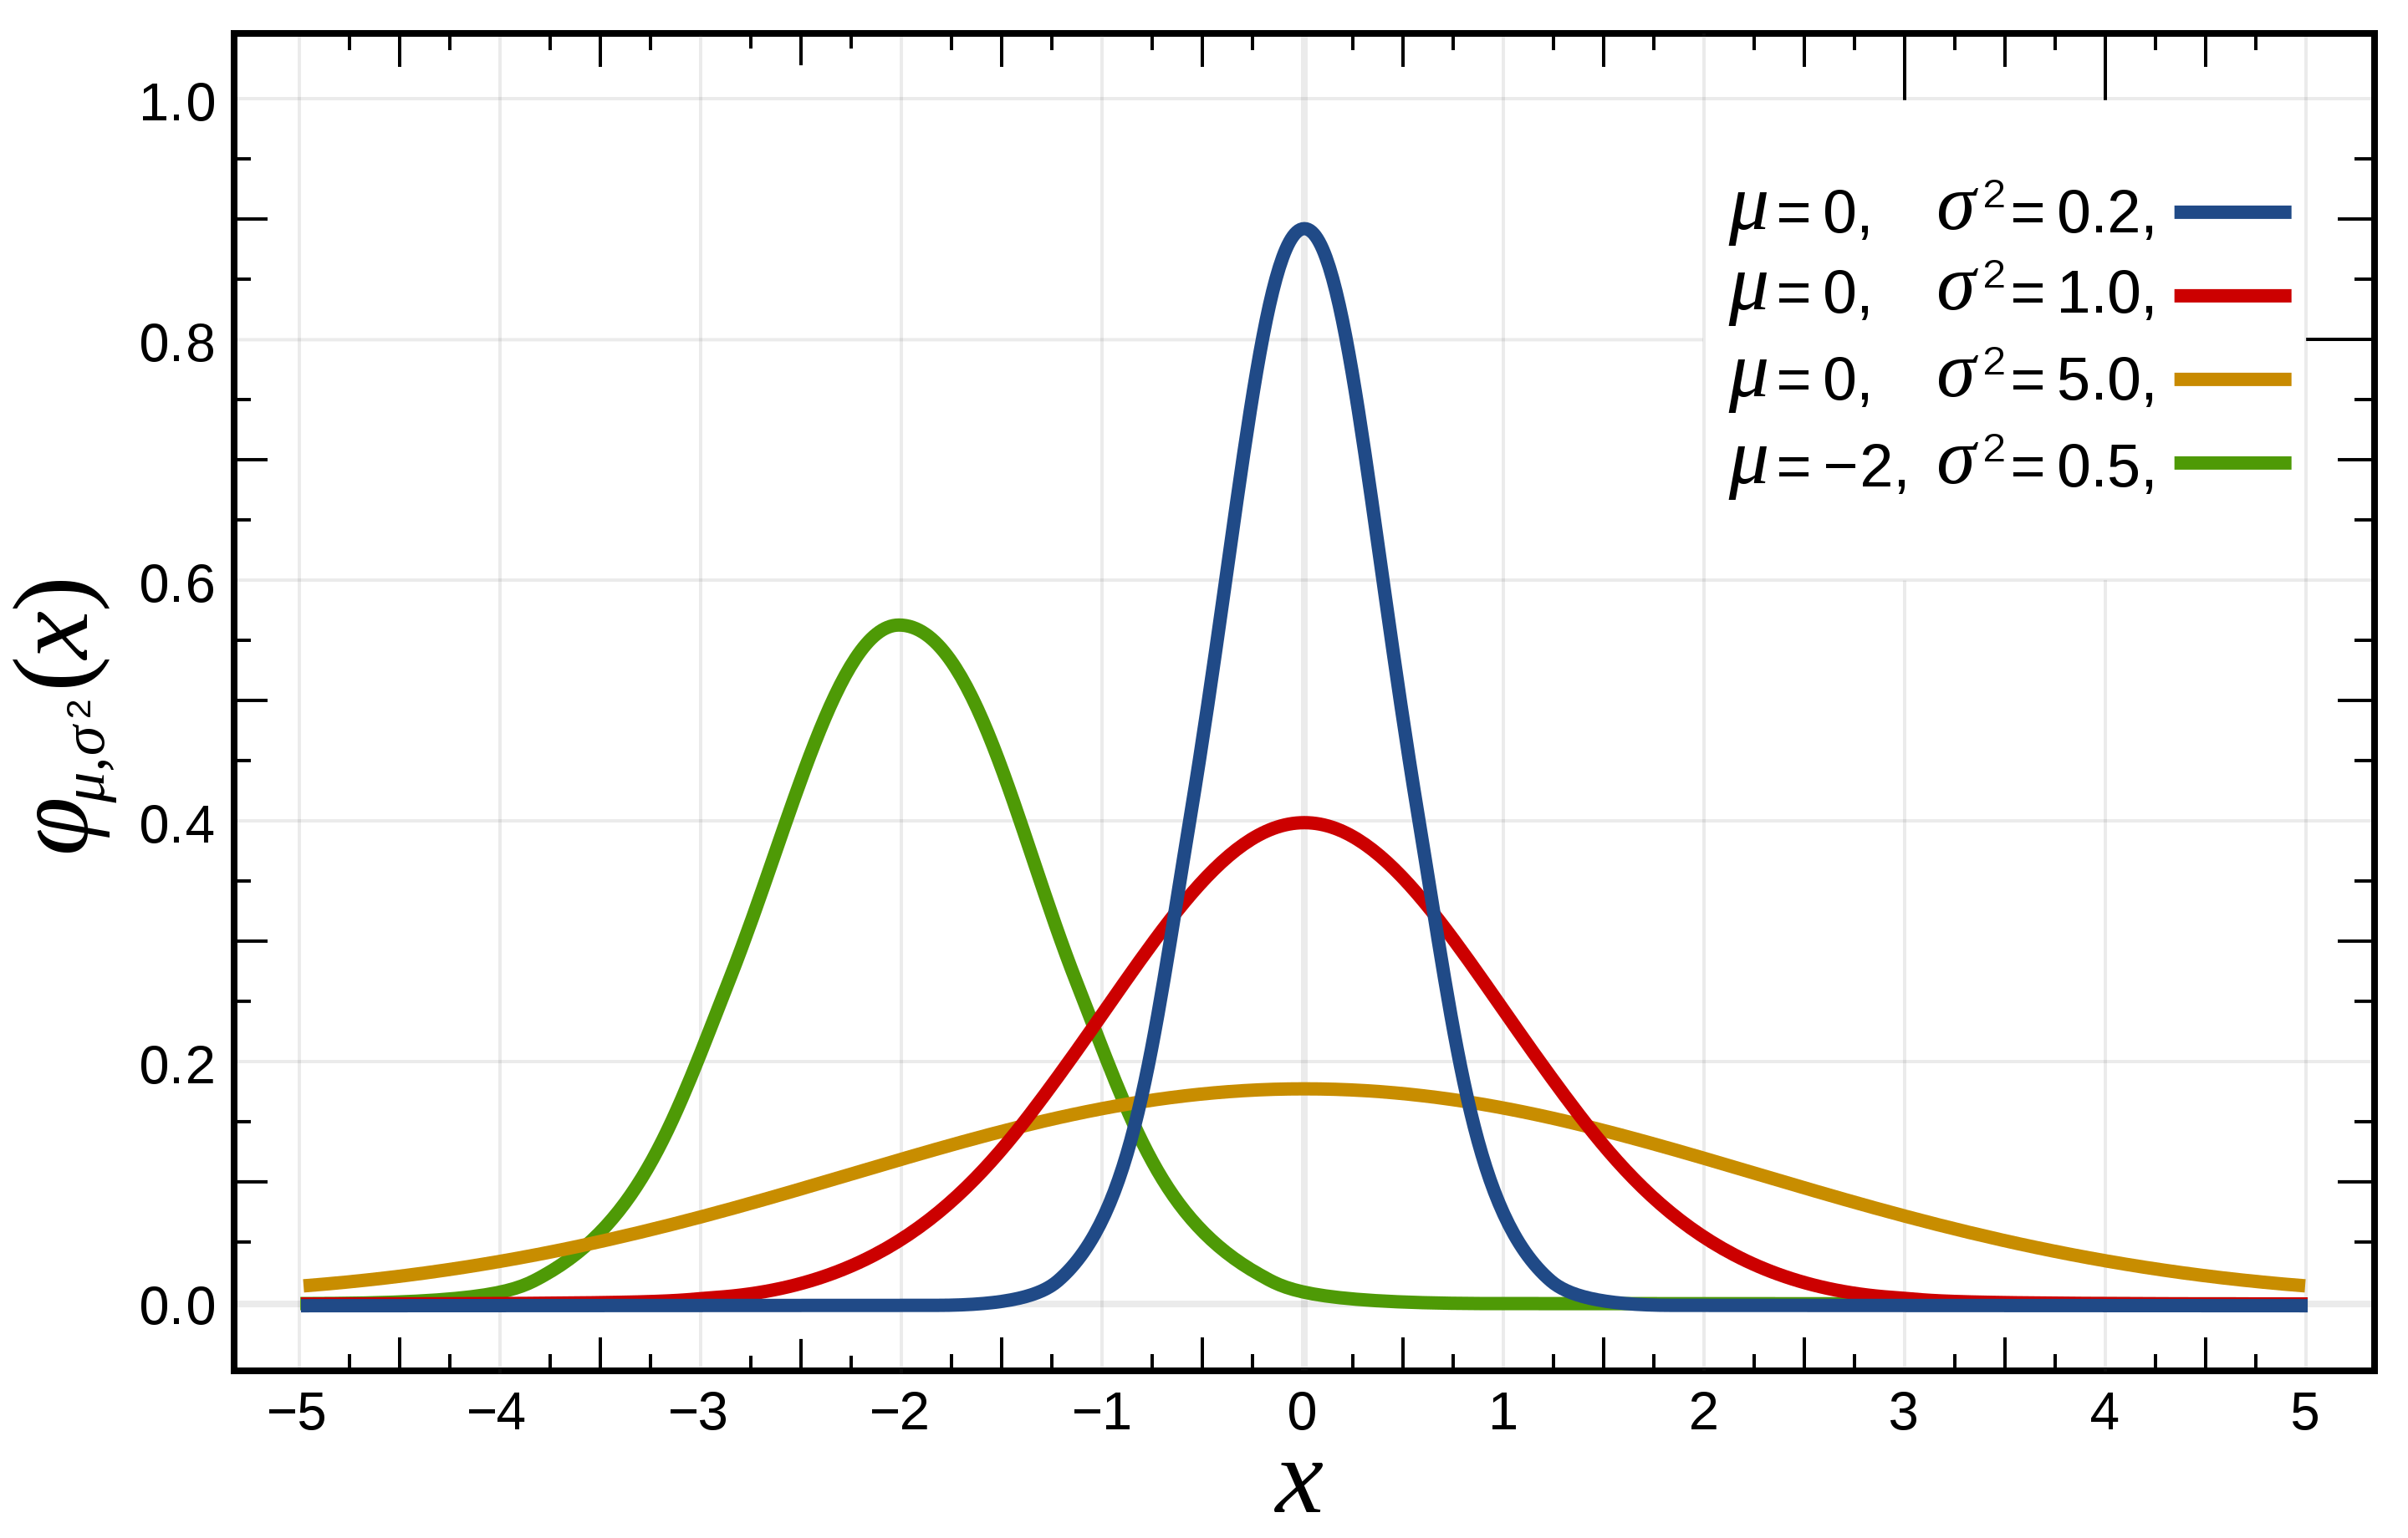
\includegraphics[width = 0.5 \textwidth]{graphic.png}
  \caption{A fancy graphic}
  \label{fg:graphic}
\end{figure}

\subparagraph{Level 5 Heading}
\lipsum[1-1][1-10]
Similar results have been reported in \cite{Kowalski2002}.

\lipsum[1-1][1-5]
Here I say something cryptic \footnote{\lipsum[1-1][1-5]}.

\lipsum[1-1][1-5]
The aformentioned principle is clearly illustrated in table~\ref{tb:raw_data}.

\begin{table}[ht]
  \centering
  \begin{tabular}{ccc}
    A & B & C \\
    \hline
    1 & 2 & 3 \\
    4 & 5 & 6 \\
    7 & 8 & 9 \\
  \end{tabular}
  \caption{Raw data}
  \label{tb:raw_data}
\end{table}

\lipsum[1-1][1-15]

\bibliography{references}

\end{document}
